\documentclass[11pt,letterpaper]{article}

\author{Jacob Thomas Errington}
\title{Assignment \#1\\Formal verification -- COMP 525}
\date{24 January 2017}

\usepackage[margin=2.0cm]{geometry}
\usepackage{amsmath,amsthm,amssymb}
\usepackage{tikz}

\usetikzlibrary{automata,arrows,positioning}

\newcommand{\ai}{\alpha_1}
\newcommand{\aii}{\alpha_2}
\newcommand{\aiii}{\alpha_3}
\newcommand{\bi}{\beta_1}
\newcommand{\bii}{\beta_2}
\newcommand{\biii}{\beta_3}

\newcommand{\hs}{\vert \vert}
\newcommand{\state}[1]{\left\langle #1 \right\rangle}

\newcommand{\locname}{\textit}

\begin{document}

\maketitle

\begin{enumerate}
    \item
        In the case of private registers and a shared variable, the possible
        outcomes of parallel computations are $2x$, $2x + 1$, $2(x + 1)$, and
        $x + 1$. Possible interleaved computations to produce each such value,
        respectively, are the following.
        \begin{itemize}
            \item $\alpha_1 \beta_1 \alpha_2 \beta_2 \alpha_3 \beta_3$ % 2x
            \item $\beta_1 \beta_2 \beta_3 \alpha_1 \alpha_2 \alpha_3$ % 2x + 1
            \item $\alpha_1 \alpha_2 \alpha_3 \beta_1 \beta_2 \beta_3$ % 2(x+1)
            \item $\alpha_1 \beta_1 \alpha_2 \beta_2 \beta_3 \alpha_3$ % x + 1
        \end{itemize}
        (The second and third executions given above are not
        interleaved, yet I fail to see how a \emph{strictly} interleaved
        execution could give rise to the value $2x + 1$ or $2(x + 1)$, so I am
        considering serial execution as a special case of interleaved
        execution.)

        In the case of a shared register and a shared variable, the possible
        values that can be computed are the same, but the executions that give
        rise to the values change. In the same order, here are example
        computations to produce the values.
        \begin{itemize}
            \item $\ai \aii \bi \bii \aiii \biii$ % 2x
            \item $\ai \bi \bii \aii \aiii \biii$ % 2x + 1
            \item $\ai \bi \aii \bii \aiii \biii$ % 2(x + 1)
            \item $\bi \bii \ai \aii \aiii \biii$ % x + 1
        \end{itemize}

    \item Figure \ref{fig:light} shows an individual traffic light, with the
        action names. Figure \ref{fig:controller} shows our simple controller.

        The parallel system $A_1 \hs A_2 \hs A_3 \hs C$ ensures by handshaking
        that no two lights are green at once, and that the order in which the
        lights become green is as required. For example, consider the initial
        state $\state{r r r r_1}$. Only the actions $R_i$ and $G_i$ are
        handshaking actions, so the lights may progress to whatever states they
        please, but they may not become green. Furthermore, the first light to
        become green must be $A_1$, since only $G_1$ is enabled in the
        controller, and all other $G_i$ are handshaking actions. The $R_i$
        actions are included in the controller to enforce that the no two
        (pairs) of lights become green simultaneously.

        \begin{figure}[ht]
            \centering
            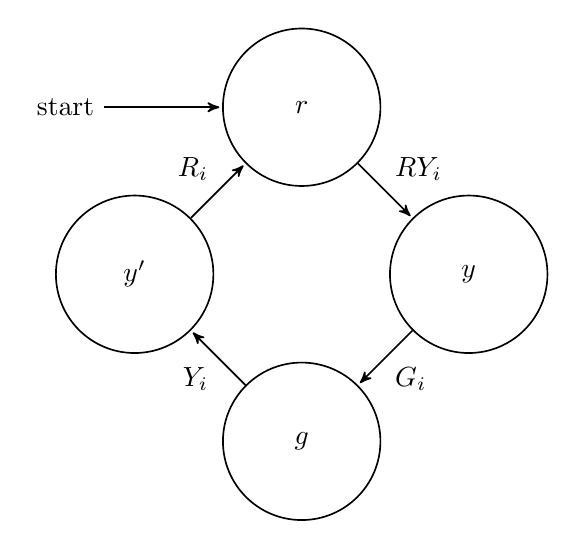
\begin{tikzpicture}[
                    ->,
                    >=stealth',
                    shorten >=1pt,
                    auto,
                    semithick,
                    node distance=3cm
                ]
                \node[] (start) {start} ;

                \begin{scope}[
                        every node/.style={minimum size=2cm, draw, circle}
                    ]
                    \node[] (red) [right of=start] {$r$} ;
                    \node[] (red-yellow) [below right of=red] {$y$} ;
                    \node[] (green) [below left of=red-yellow] {$g$} ;
                    \node[] (yellow) [above left of=green] {$y^\prime$} ;
                \end{scope}

                \path
                (start) edge node {} (red)
                (red) edge node {$RY_i$} (red-yellow)
                (red-yellow) edge node {$G_i$} (green)
                (green) edge node {$Y_i$} (yellow)
                (yellow) edge node {$R_i$} (red)
                ;
            \end{tikzpicture}
            \caption{
                The $i$\textsuperscript{th} traffic light (pair). The actions
                are mnemonics based on the state that is transitioned into.
                Furthmore, each action is indexed by the light number.
                Hence, actions are distinct across all lights, but there is
                some overlap with the actions used in the controller.
            }
            \label{fig:light}
        \end{figure}

        \begin{figure}[ht]
            \centering
            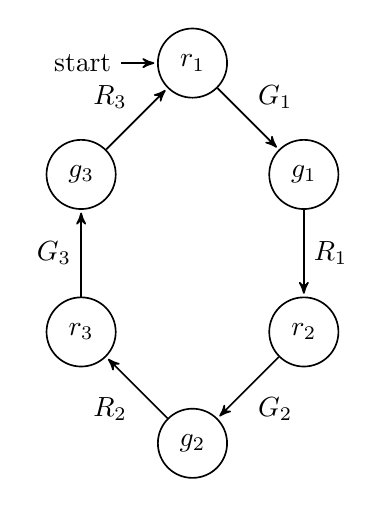
\begin{tikzpicture}[
                    ->,
                    >=stealth',
                    shorten >=1pt,
                    auto,
                    semithick,
                    node distance=2cm
                ]
                \node[initial, state] (pre-g-1) {$r_1$} ;
                \node[state] (g-1) [below right of=pre-g-1] {$g_1$} ;
                \node[state] (pre-g-2) [below of=g-1] {$r_2$} ;
                \node[state] (g-2) [below left of=pre-g-2] {$g_2$} ;
                \node[state] (pre-g-3) [above left of=g-2] {$r_3$} ;
                \node[state] (g-3) [above of=pre-g-3] {$g_3$} ;

                \path
                (g-3) edge node {$R_3$} (pre-g-1)
                (pre-g-1) edge node {$G_1$} (g-1)
                (g-1) edge node {$R_1$} (pre-g-2)
                (pre-g-2) edge node {$G_2$} (g-2)
                (g-2) edge node {$R_2$} (pre-g-3)
                (pre-g-3) edge node {$G_3$} (g-3)
                ;
            \end{tikzpicture}
            \caption{
                A simple ``reasonable'' controller for the traffic light system
                that ensures that lights become green in a loop with the order
                $A_1$, $A_2$, $A_3$.
            }
            \label{fig:controller}
        \end{figure}

    \item
        The first candidate solution to the mutual exclusion problem is not
        correct: both processes might enter their critical sections
        simultaneously. Label the $i$\textsuperscript{th} line of code of
        process $1$ by $\alpha_i$ and of process $2$ by $\beta_i$.
        An execution sequence starting out with $\ai \bi$ will result in both
        processes entering their critical sections at the same time, which
        violates the principle of the critical section.

        The second candidate solution to the mutual exclusion problem is
        correct. Suppose both processes are in their critical sections at the
        same time. This would require that $c_1 = c_2 = 1$ in order for both of
        the \texttt{if}-statements to pass. However, $c_1$ has the value $1$
        only after the end of its critical section of process $1$ and
        $\alpha_1$. Hence we arrive at a contradiction.

        The second candidate solution suffers from the possibility of deadlock.
        Consider the execution sequence beginning by $\alpha_1 \beta_1$.
        Process $1$ now waits for process $2$ to complete its critical section
        (to set $c_2 = 1$) and vice versa. This situation of \emph{circular
        wait} prevents overall progress from being made in either process.

    \item Now we consider Dekker's solution to the mutual exclusion problem.

        \begin{description}
            \item[Correctness.]
                Notice that while process $1$ is in its critical section,
                $c_1 = 0$. Suppose that process $1$ is in its critical section.
                Suppose that process $2$ enters its critical section. This
                would require that $c_1 = 1$, which is a contradiction.

            \item[Deadlock-free.]
                The only execution sequences that might be problematic are
                those in which $c_1 = c_2 = 0$ and both processes arrive at
                \texttt{L1}, \texttt{L2} simultaneously. Suppose without loss
                of generality that \texttt{turn = 1}. Then process $2$ will set
                $c_2 = 1$ (indicating that it no longer wants to enter the
                critical section as it has discovered that it is not its turn)
                and process $1$ will loop back to the contention check
                \texttt{if c2 = 0}. It will discover that there is no more
                contention and proceed to execute its critical section, hence
                unblocking process 2 by setting \texttt{turn = 2} (process $2$
                has been busy waiting for this to occur). Process $2$ will then
                loop to its beginning, indicate that it would like to enter the
                critical section, and by a symmetrical argument be guaranteed
                to enter its critical section even in case of contention.

            \item[Starvation-free.]
                Notice that the turn variable is only consulted in case of
                contention for entry to the critical section. Consequently, one
                process may decide it no longer wants to enter its critical
                section anymore (i.e. it never leaves its non-critical section)
                and the other process will be able to enter the critical
                section as much as it likes.

                Contention, if any, is resolved \emph{fairly} by the
                alternation of the \texttt{turn} variable at the end of the
                critical section. Upon completion of one process's critical
                section, the other process becomes guaranteed to enter its
                critical section in finite time only \emph{should it want to}.
        \end{description}

    \item
        Figure \ref{fig:pg} shows the program graph of process $1$. Figure
        \ref{fig:tspg} shows the transition system semantics of the
        interleaved program graphs of process $1$ and $2$.

        The transition system is infinite. This is easy to see by considering
        the execution $\state{NC,NC}\state{W,NC}\state{CS,NC}\state{NC,NC}$
        which forms a loop that may be repeated indefinitely. (We omit the
        evaluation components of these states since they are uniquely
        determined.)

        Next we claim that the algorithm ensures mutual exclusion. Suppose that
        both processes are in their critical sections at once. Then by the
        guards we infer both $y_2 = 0 \lor y_1 < y_2$
        and $y_1 = 0 \lor y_2 < y_1$. Note that prior to entering their
        critical sections, assignments to $y_1$ and $y_2$ are made in one of
        two possible orders. Either way, the values of these variables
        necessarily become nonzero. Hence, the cases $y_1 = 0$ and $y_2 = 0$ in
        the disjunctions are impossible. Finally we infer that $y_1 < y_2
        \land y_2 < y_1$ which is a contradiction.

        Next we claim that the algorithm does not deadlock. Suppose that both
        processes are in the waiting state. Then the assignments to the
        variables $y_1$ and $y_2$ occurred in some order. These assignments
        necessarily ensure that neither variable has the value $0$. The order
        in which those operations occur determines which of $y_1$ or $y_2$ is
        minimal. Hence, the guard of one of the processes will be satisfied and
        progress will be made. This means that no deadlock occurs.

        Next we claim that the algorithm prevents starvation. Suppose without
        loss of generality that process $1$ wants to enter its critical
        section. Some cases arise. First, it may have raced process $2$ to
        arrive at the \texttt{wait} instruction. In this case, the result of
        the race will determine which of the variables is minimal and hence
        which process may enter its critical section. If process $1$ wins the
        race, then it enters and we're done. Otherwise, process $1$ blocks
        while process $2$ is in its critical section. Once process $2$ exits
        its critical section, it executes $y_2 \gets 0$ to signal that it is no
        longer wants to enter its critical section. If process $2$ never wishes
        to enter its critical section again, then the variable $y_2$ will
        remain with the value $0$, and process $1$'s guard will be satisfied
        allowing it to enter its critical section. If process $1$ ``zips
        around'' to its \texttt{wait} instruction before process $1$'s
        \texttt{wait} instruction wakes up (we assume a polling
        implementation), then $y_2 > y_1$. Hence, process $1$'s guard will be
        satisfied, allowing it to enter its critical section. Hence, if process
        $1$ wants to enter its critical section, it will enter it within a
        finite amount of time. By symmetry, the same applies to process $2$.

        \begin{figure}[ht]
            \centering
            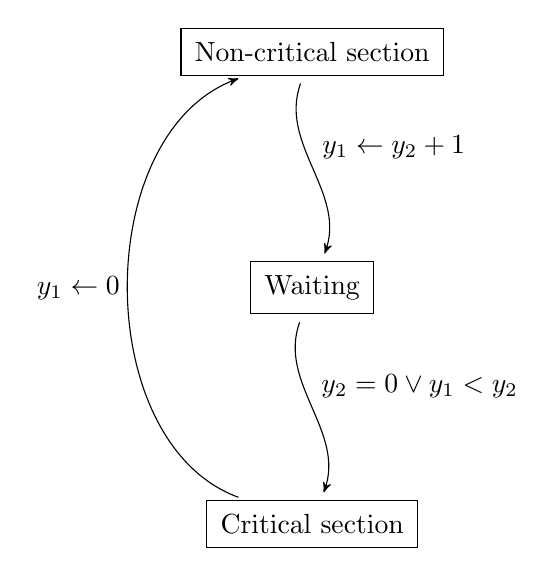
\begin{tikzpicture}[
                    location/.style={
                        rectangle,
                        draw=black,
                        inner sep=0.5em
                    },
                    node distance=3cm,
                    ->,
                    shorten >=3pt,
                    shorten <=3pt,
                    >=stealth',
                    auto
                ]
                \node (NC) [location] {Non-critical section};
                \node (W) [location, below of=NC] {Waiting};
                \node (CS) [location, below of=W] {Critical section};

                \draw [->] (NC) to [out=250, in=70] node {$y_1 \gets y_2 + 1$} (W);
                \draw [->] (W) to [out=250, in=70] node {$y_2 = 0 \lor y_1 < y_2$} (CS);
                \draw [->] (CS) to [out=160, in=200] node {$y_1 \gets 0$} (NC);
            \end{tikzpicture}

            \caption{
                The program graph of process $1$. Notice that the arrow between
                the \locname{Waiting} and the \locname{Critical section}
                locations is labelled with a guard, whereas the other arrows
                are labelled with side-effects.
            }
            \label{fig:pg}
        \end{figure}

        \begin{figure}[ht]
            \centering
            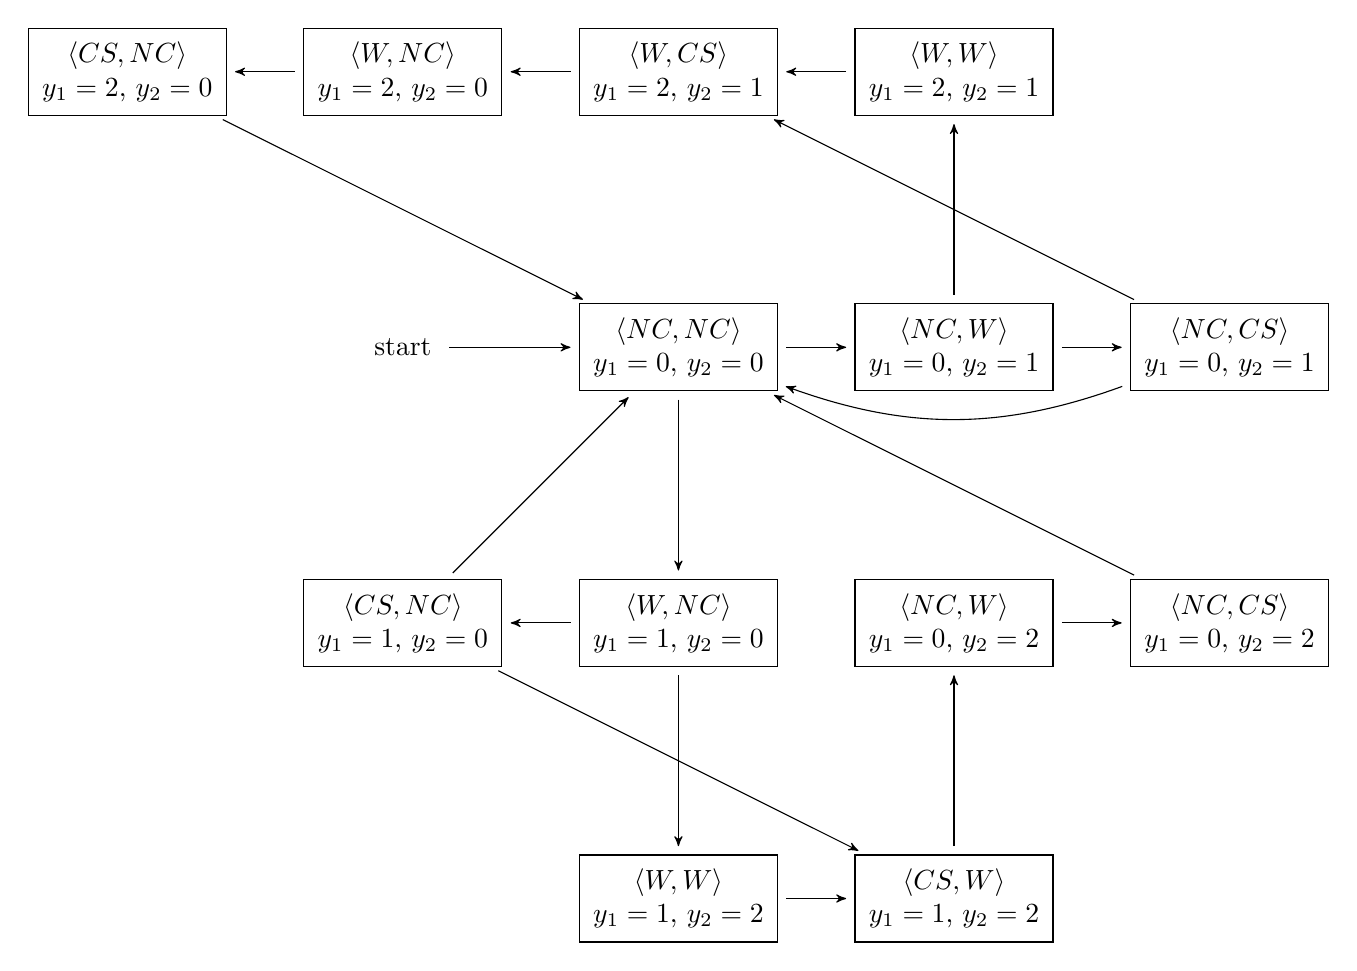
\begin{tikzpicture}[
                    location/.style={
                        rectangle,
                        draw=black,
                        inner sep=0.5em,
                        align=center
                    },
                    node distance=3.5cm,
                    ->,
                    shorten >=3pt,
                    shorten <=3pt,
                    >=stealth',
                    auto
                ]
                \newcommand{\mkstate}[6]{
                    \node (#1) [location,#6] {
                        $\state{#2,#3}$ \\ $y_1 = #4$, $y_2 = #5$
                    };
                }
                \mkstate{NCNC00}{NC}{NC}{0}{0}{}
                \mkstate{WNC10}{W}{NC}{1}{0}{below of=NCNC00}
                \mkstate{CSNC10}{CS}{NC}{1}{0}{left of=WNC10}

                \mkstate{NCW01}{NC}{W}{0}{1}{right of=NCNC00}
                \mkstate{WW12}{W}{W}{1}{2}{below of=WNC10}
                \mkstate{CSW12}{CS}{W}{1}{2}{right of=WW12}

                \mkstate{NCW02}{NC}{W}{0}{2}{above of=CSW12}
                \mkstate{NCCS02}{NC}{CS}{0}{2}{right of=NCW02}

                \mkstate{WW21}{W}{W}{2}{1}{above of=NCW01}
                \mkstate{WCS21}{W}{CS}{2}{1}{left of=WW21}
                \mkstate{WNC20}{W}{NC}{2}{0}{left of=WCS21}

                \mkstate{NCCS01}{NC}{CS}{0}{1}{right of=NCW01}
                \mkstate{CSNC20}{CS}{NC}{2}{0}{left of=WNC20}

                \node (start) [left of=NCNC00] {start};
                \path
                (start) edge (NCNC00)
                ;

                \path
                (NCNC00) edge (WNC10)
                (WNC10) edge (CSNC10)
                (CSNC10) edge (NCNC00)

                (NCNC00) edge (NCW01)
                (NCW01) edge (WW21)
                (WW21) edge (WCS21)
                (WNC20) edge (CSNC20)
                (CSNC20) edge (NCNC00)

                (WNC10) edge (WW12)
                (WW12) edge (CSW12)
                (CSW12) edge (NCW02)
                (NCCS02) edge (NCNC00)

                (WCS21) edge (WNC20)
                (NCW02) edge (NCCS02)
                (NCW01) edge (NCCS01)
                (NCCS01) edge [out=200, in=340] (NCNC00)
                (NCCS01) edge (WCS21)
                (CSNC10) edge (CSW12)
                ;
            \end{tikzpicture}
            \caption{
                The transition system representation of the interleaved program
                graphs, guarded globally by $y_1 \leq 2$ and $y_2 \leq 2$.
                Unreachable states are omitted. We leave the arrows unlabelled
                since the action may be inferred from the change in the
                evaluation.
            }
            \label{fig:tspg}
        \end{figure}
\end{enumerate}

\end{document}
